%(BEGIN_QUESTION)
% Copyright 2006, Tony R. Kuphaldt, released under the Creative Commons Attribution License (v 1.0)
% This means you may do almost anything with this work of mine, so long as you give me proper credit

På jobb blir du sendt for å feilsøke et helt nytt reguleringssystem, bestående av en pneumatisk nivåsender koblet til en pneumatisk regulator, som igjen styrer en pneumatisk reguleringsventil. Prosesskar, rør, ventil, regulator og nivåsender er alle helt nye, med fersk maling.

$$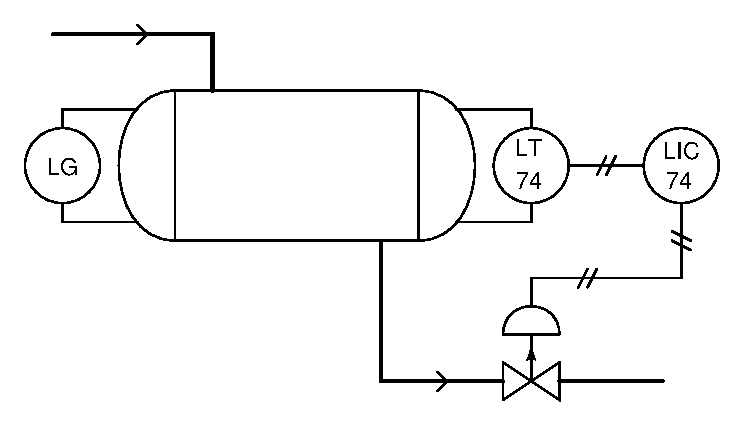
\includegraphics[width=15.5cm]{i00140x01.eps}$$

Ifølge operatøren har dette nivåsystemet {\it aldri} fungert. Væskenivået i karet er så lavt at nivåglasset (LG) står tomt, men regulatoren kommanderer ventilen til 100\% åpen, som naturligvis fortsetter å tømme karet og hindrer nivåoppbygging.

Siden du kan reguleringsteori, sjekker du hvordan regulatoren er konfigurert. Inne i regulatoren ser du at den står i {\it direkte} virkning: økende PV gir økende utgangssignal (MV), som flytter luft-til-lukke-ventilen mer mot «lukket».

Du forstår hvordan problemet skal løses, og flytter en intern spak i regulatoren til {\it revers} virkning.

\vskip 10pt

Forklar hvorfor dette løser problemet.

\vskip 20pt \vbox{\hrule \hbox{\strut \vrule{} {\bf Forslag til sokratisk diskusjon} \vrule} \hrule}

\begin{itemize}
\item{} Forklar betydningen av at systemet er «nytt». Hvordan ville antakelsene dine vært annerledes hvis anlegget var gammelt og rustent?
\item{} Hvordan tror du regulatoren ble feilkonfigurert i utgangspunktet?
\item{} Hva måtte vært annerledes i systemet for at direktevirkende regulator kunne vært riktig i stedet for revers?
\item{} Hvis du ikke hadde oppdaget direktevirkende innstilling: kunne det forklart symptomene dersom regulatoren sto i manuell modus i stedet for automatisk?
\end{itemize}

\underbar{file i00140}
%(END_QUESTION)





%(BEGIN_ANSWER)


%(END_ANSWER)





%(BEGIN_NOTES)

Dette var et faktisk problem jeg møtte i en jobb på et oljeraffineri.

\vskip 10pt

Et godt diagnostisk prinsipp er å spørre hvor {\it nytt} et feilende system er. Feil i gamle systemer har ofte annen karakter enn feil i helt nye systemer. Fersk maling på kar og rør er et viktig hint: når systemet er så nytt, har det {\it sannsynligvis aldri fungert riktig}, og feilen er ofte en form for feilkonfigurasjon. I dette tilfellet var feilen feil regulatorvirkning.

Feil i gamle (tidligere fungerende) systemer skyldes oftere slitasje enn feilkonfigurasjon. Selvsagt kan noen feilkonfigurere et instrument i et system som har virket i årevis, men det er mindre sannsynlig, fordi slike feil ofte gir umiddelbare symptomer og blir raskt rettet av den som gjorde endringen.

Samme regel gjelder for eldre systemer som nylig er bygd om. Når en prosess eller maskin ikke oppfører seg normalt rett etter ombygging, skyldes det oftest feil konfigurering eller feil installasjon, ikke komponentaldring.

\vskip 20pt \vbox{\hrule \hbox{\strut \vrule{} {\bf Virtuell feilsøking} \vrule} \hrule}

Dette spørsmålet egner seg godt som en «virtuell feilsøking»-øvelse. Når du presenterer diagrammet for studentene, ser du først for deg en bestemt feil i systemet. Deretter presenterer du ett eller flere symptomer på feilen (noe en operatør eller annen bruker kan observere). Studentene foreslår så diagnostiske tester for å finne feiltype og feilsted, som om de var teknikere i feilsøking. Din jobb er å oppgi hvilke resultater disse testene ville gitt, og dokumentere resultatene synlig for alle studentene.

Under og etter øvelsen er det nyttig å stille oppfølgingsspørsmål som:

\begin{itemize}
\item{} Hva forteller resultatet av siste diagnostiske test om feilen?
\item{} Anta at resultatet av siste test var annerledes. Hva ville det da fortalt om feilen?
\item{} Er siste diagnostiske test den beste vi kunne gjort?
\item{} Hva ville vært ideell testrekkefølge for å finne feilen i færrest mulig steg?
\end{itemize}



\vfil \eject

\noindent
{\bf Forhåndsquiz:}

{\it Direkte virkning} for en prosessregulator er definert som:

\begin{itemize}
\item{} Prosessvariabelsignalet (PV) øker når settpunktsignalet (SP) øker
\vskip 5pt
\item{} Prosessvariabelsignalet (PV) synker når settpunktsignalet (SP) øker
\vskip 5pt
\item{} Utgangssignalet (MV) synker når prosessvariabelen (PV) øker
\vskip 5pt
\item{} Utgangssignalet (MV) øker når prosessvariabelen (PV) øker
\vskip 5pt
\item{} Settpunktsignalet (SP) øker når prosessvariabelen (PV) øker
\vskip 5pt
\item{} Settpunktsignalet (SP) synker når prosessvariabelen (PV) øker
\end{itemize}


\vfil \eject

\noindent
{\bf Forhåndsquiz:}

{\it Revers virkning} for en prosessregulator er definert som:

\begin{itemize}
\item{} Prosessvariabelsignalet (PV) øker når settpunktsignalet (SP) synker
\vskip 5pt
\item{} Prosessvariabelsignalet (PV) synker når settpunktsignalet (SP) synker
\vskip 5pt
\item{} Utgangssignalet (MV) synker når prosessvariabelen (PV) øker
\vskip 5pt
\item{} Utgangssignalet (MV) øker når prosessvariabelen (PV) øker
\vskip 5pt
\item{} Settpunktsignalet (SP) øker når prosessvariabelen (PV) øker
\vskip 5pt
\item{} Settpunktsignalet (SP) synker når prosessvariabelen (PV) øker
\end{itemize}


%INDEX% Basics, control loop troubleshooting: determining cause of control problem
%INDEX% Process: receiver vessel liquid level control (generic)

%(END_NOTES)
